\documentclass[pdftex,12pt,a4paper]{article}

\usepackage{wrapfig,amssymb,amsmath,graphicx, subfigure}
\usepackage[dutch]{babel}
\usepackage[top=0.5in, bottom=0.5in, left=1in, right=1in]{geometry}
\pagenumbering{arabic}
\newcommand{\HRule}{\rule{\linewidth}{0.5mm}}

\begin{document}
\begin{titlepage}

% Upper part of the page
\begin{flushleft}

\includegraphics[trim=23mm 0mm 0mm 0mm, width=1\textwidth]{./logo.jpg}\\[1cm] \end{flushleft}
\begin{center}
	\textsc{\Large Netcentric Computing}\\[0.5cm]

    % Title
    \HRule \\[0.4cm] { \huge \bfseries Report for first week assignment}\\[0.4cm]

    \HRule \\[1.5cm]

    % Author and supervisor
\begin{minipage}{0.4\textwidth}
\begin{flushleft} \large \emph{Authors:}\\
Jaap \textsc{Koetsier}\\
Jelte \textsc{Fennema}\\
Abe \textsc{Wiersma}\\
\end{flushleft}
\end{minipage}
\begin{minipage}{0.4\textwidth} \begin{flushright} \large \end{flushright}\end{minipage}

    \vfill

    % Bottom of the page 
    {\large \today}

\end{center}
\end{titlepage}
\pagebreak
\section{Servo naar Mbed}
De stap van de servo naar de embed ging eigenlijk vrij gemakkelijk, binnen het eerste uur van spelen met de embed software hadden we al uitgevonden hoe de data uitgelezen zou moeten worden. Na een hoop gespeel met voltages kwamen we erachter dat de standen van de potentiometer gekalibreerd zouden moeten worden, van 0 t/m 10 (0.0, 0.005, 0.0215, 0.06, 0.104, 0.149, 0.199, 0.2985, 0.513, 0.76, 0.998).
Bij deze standen bepaalden we ook een precisie opdat de motor stil zou staan op een bepaalde stand, er zit een bepaalde variatie binnen de stilstaande voltage van de potentiometer(0.0005, 0.0005, 0.00075, 0.0015, 0.0025, 0.0025, 0.003, 0.0035, 0.0035, 0.004, 0.001).
Voor interactie met de motor, verbonden aan de mbed, gebruikten we de Hbridge library. Deze library is makkelijk gebruikbaar en van een HBridge object gebruiken we slechts 2 functies, hbridge.power(true). En hbridge.speed([-1.0 - 1.0]) om de richting en snelheid van de motor te bepalen.


\section{Mbed naar Android Telefoon}
Omdat we eerst de Mbed aan de computer hadden verbonden en daarin een message passing systeem hadden geimplementeerd was de stap naar Mbed tot Android Phone vrij klein.

De Mbed ontvangt een string die door strtof naar een int probeert te worden omgevormd, wanneer dit lukt wordt command active flag op $1$ gezet en wordt er naar de doorgegeven positie gedraaid door de motor in de servo. De command active flag geeft in de tick, de \' while\' loop binnen de ADK library, aan dat er bewogen moet worden.

In deze zelfde tick wordt elke iteratie van de positie van de servo doorgegeven naar de android telefoon verbonden met de Mbed. Deze positie wordt in gehele procenten meegegeven. Omdat de potentiometer geen lineair pad volgt hebben we paden tussen de gehele punten op de potentiometer lineair geinterpoleert, zie hieronder.\\
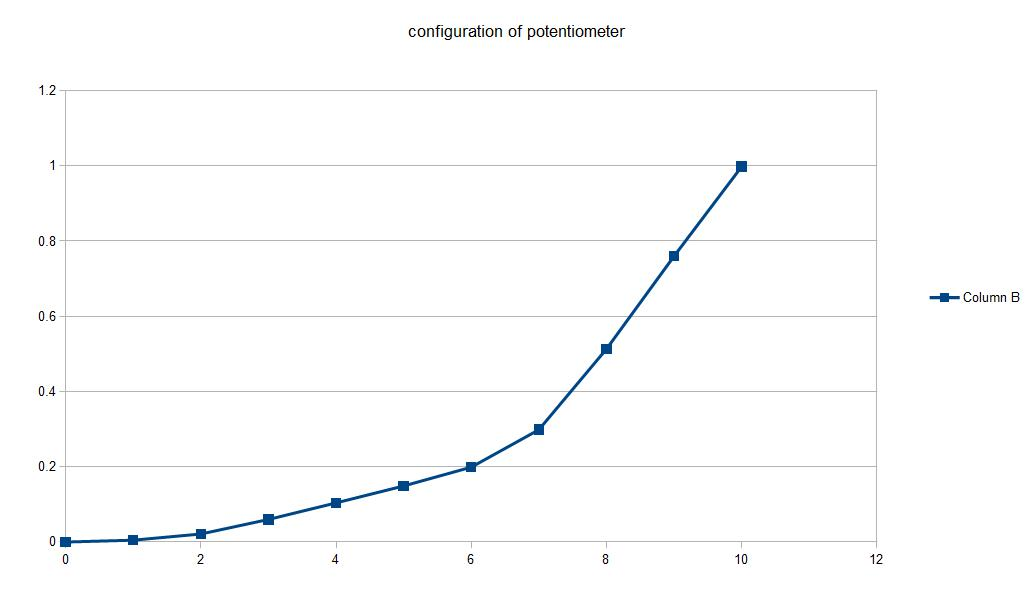
\includegraphics[width=1\textwidth]{./calibration.jpg}\\
De mbed interpreteert het voltage afkomstig uit de servo als een getal tussen 0 en 1, waarbij 0 staat voor 0 volt en 1 staat voor de volle 3.3V.

\section{Android naar Android (Bluetooth)}
Nadat we met de Android applicatie de mbed aan konden sturen hebben we ons
gericht op de bluetooth-implementatie. Omdat wij niet gezien hadden dat er een
werkend framework aangeboden was (deze stond onder een link "Android Studio",
welke wij al geinstalleerd hadden, en zodoende niet aangeklikt hadden) hebben we
onze eigen applicaties vanuit niets opgebouwd: een applicatie die dient als
bluetoothserver en een bluetooth client. De applicatie die dient als
server neemt de communicatie met de mbed voor zijn rekening, de bluetooth client
applicatie maakt verbinding met de server en stuurt de gewenste stand van de
servo door naar de server.\\
Het programmeren van de bluetooth-communicatie zelf is in Android vrij eenvoudig,
de online documentatie geeft een duidelijk stappenplan met voorbeeldcode, die we
eenvoudig aan onze eigen wensen aan konden passen. Een connectie tussen de twee
applicaties was zonder veel moeite opgezet: Het enige probleem dat we hier zijn
tegengekomen (en ons toch een paar uur gekost heeft) is dat - om een voor ons
onbekende reden - een bepaalde random UUID die we gebruikten voor de connectie
niet werkte, ondanks dat deze op beide apparaten hetzelfde was. Hier kwamen we
achter nadat we een lijst van beschikbare UUID's van een laptop opvroegen en
deze verbinding moeiteloos tot stand kwam.\\
Het grootste probleem bij het versturen van data over de bluetooth-connectie was
onze worsteling met Android zelf; het versturen van data uit onze main Activity
(waar een SeekBar in staat waarmee we integers genereren om uiteindelijk de
servo aan te sturen) naar de thread waarin de bluetooth-verbinding loopt. We
hebben op 1001 manieren geprobeerd messages door te sturen via Handlers, die we
op verschillende creatieve manieren weer tussen activities and threads hebben
proberen door te sturen, maar door onze gebrekkige kennis van Android wilde dit
niet lukken. Uiteindelijk hebben we een Service aangemaakt waarin we de
referentie naar de ConnectedThread gezet hebben. Services zijn vanuit alle 
activities te benaderen, dus hierdoor was het eenvoudig de write() functie uit
de ConnectedThread instantie aan te roepen.\\

\section{Conclusie}
Helaas hebben we de servo niet met meerdere clients aan kunnen sturen, doordat
we vrijdagmiddag een uur voordat het lokaal dichtging pas via een ander groepje
te horen kregen dat er nog een ander framework was. Hier zijn we even mee bezig
geweest, maar in dat uurtje zijn we niet zover gekomen dat het ook werkte.
Aangezien we in het weekend niet de beschikking hadden over de mbed hebben we
ervoor gekozen de applicaties af te maken waar we mee begonnen waren, omdat
hierin de mbed-besturing al werkte. Zodra we de bluetooth-verbinding werkende
hadden zou het alleen nog een kwestie zijn van het doorsturen van de ontvangen
waarde naar de mbed. Dit is hoe we het uiteindelijk gedaan hebben. De combinatie
bluetooth/mbed hebben we dus niet kunnen testen, maar we kunnen met aan waarheid
grenzende waarschijnlijkheid zeggen dat dit werkt, omdat het slechts een kwestie
is van de bron van de variabele waarmee we de functie aanroepen.\\


\section{Diagram}
Hieronder valt het diagram te vinden dat in vrij grote precisie onze opstelling representeerd.\\
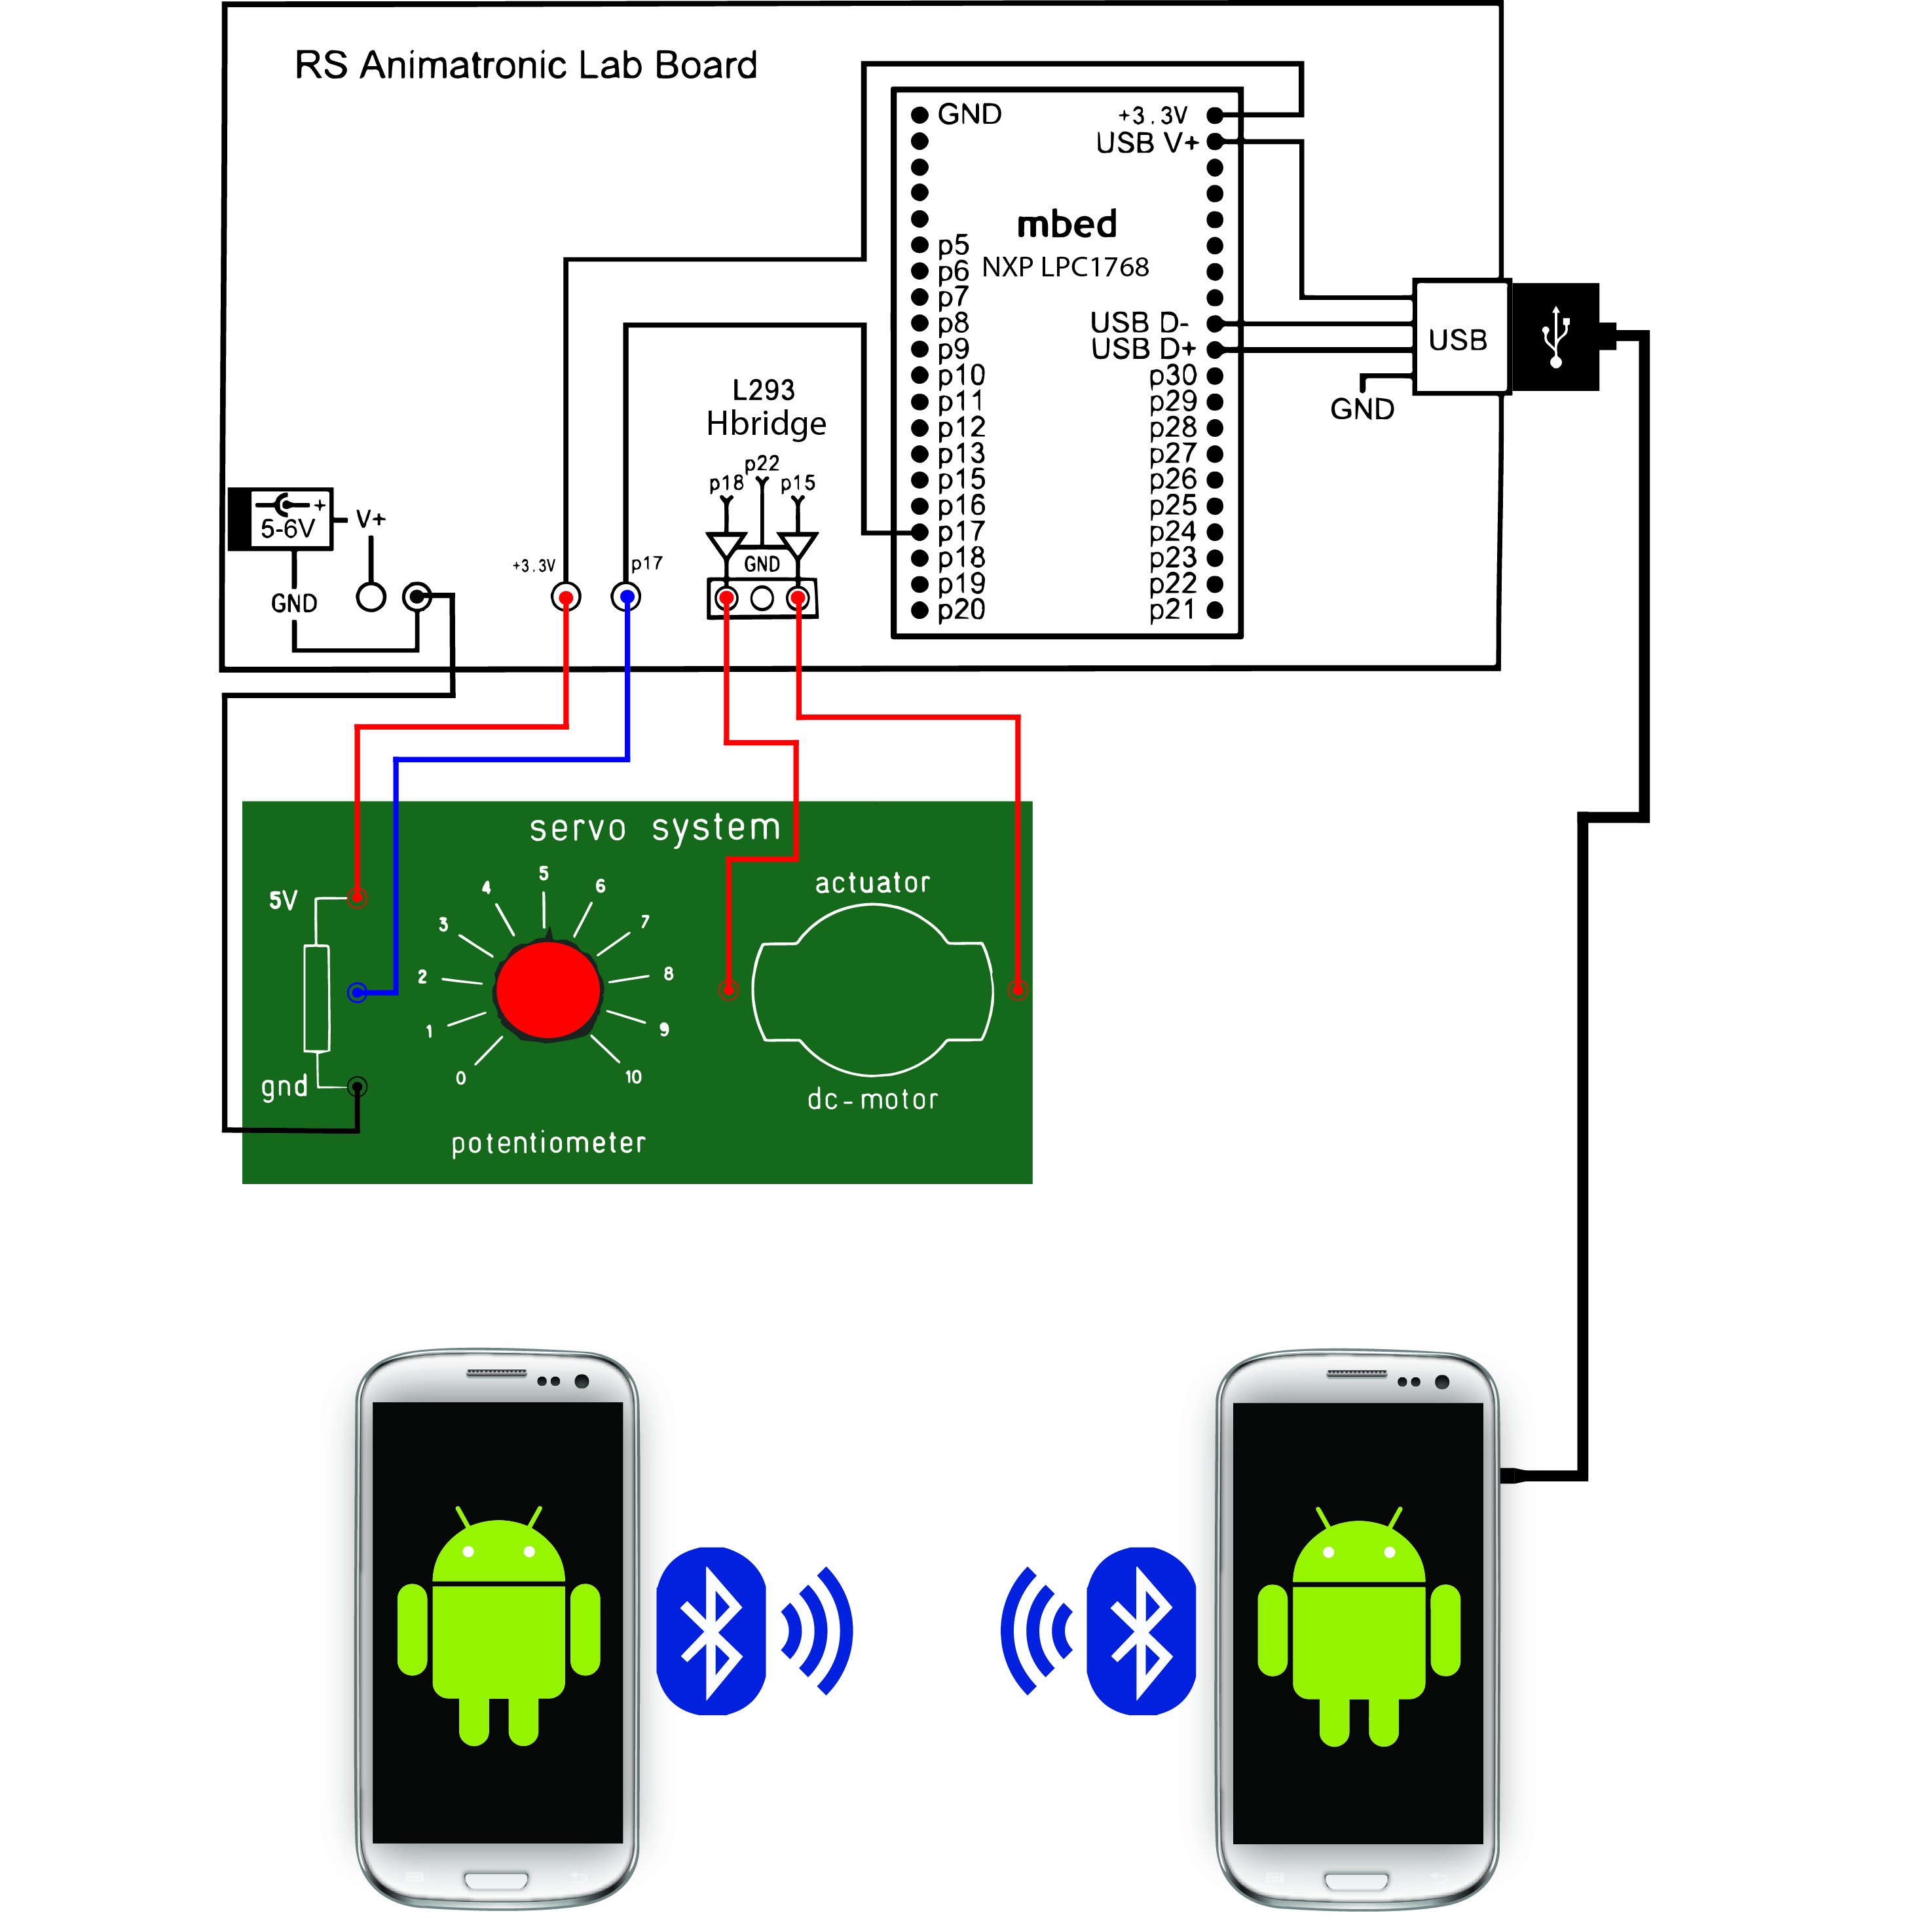
\includegraphics[width=1\textwidth]{./diagram.jpg}\\
\end{document}